\section{Modelo Relacional}

El modelo relacional representa la estructura lógica de la base de datos del sistema \textbf{QuickContentMedia}. Define las entidades, atributos y relaciones que permiten almacenar y gestionar la información del sistema de manera estructurada.

\subsection{Diagrama del Modelo Relacional}
La figura \ref{fig:DiagramaModeloRelacional} muestra el diagrama del modelo relacional del sistema \textbf{QuickContentMedia}. Este diagrama fue elaborado utilizando la herramienta Visual Paradigm~\cite{staruml2024}.

\begin{figure}[H]
    \centering
    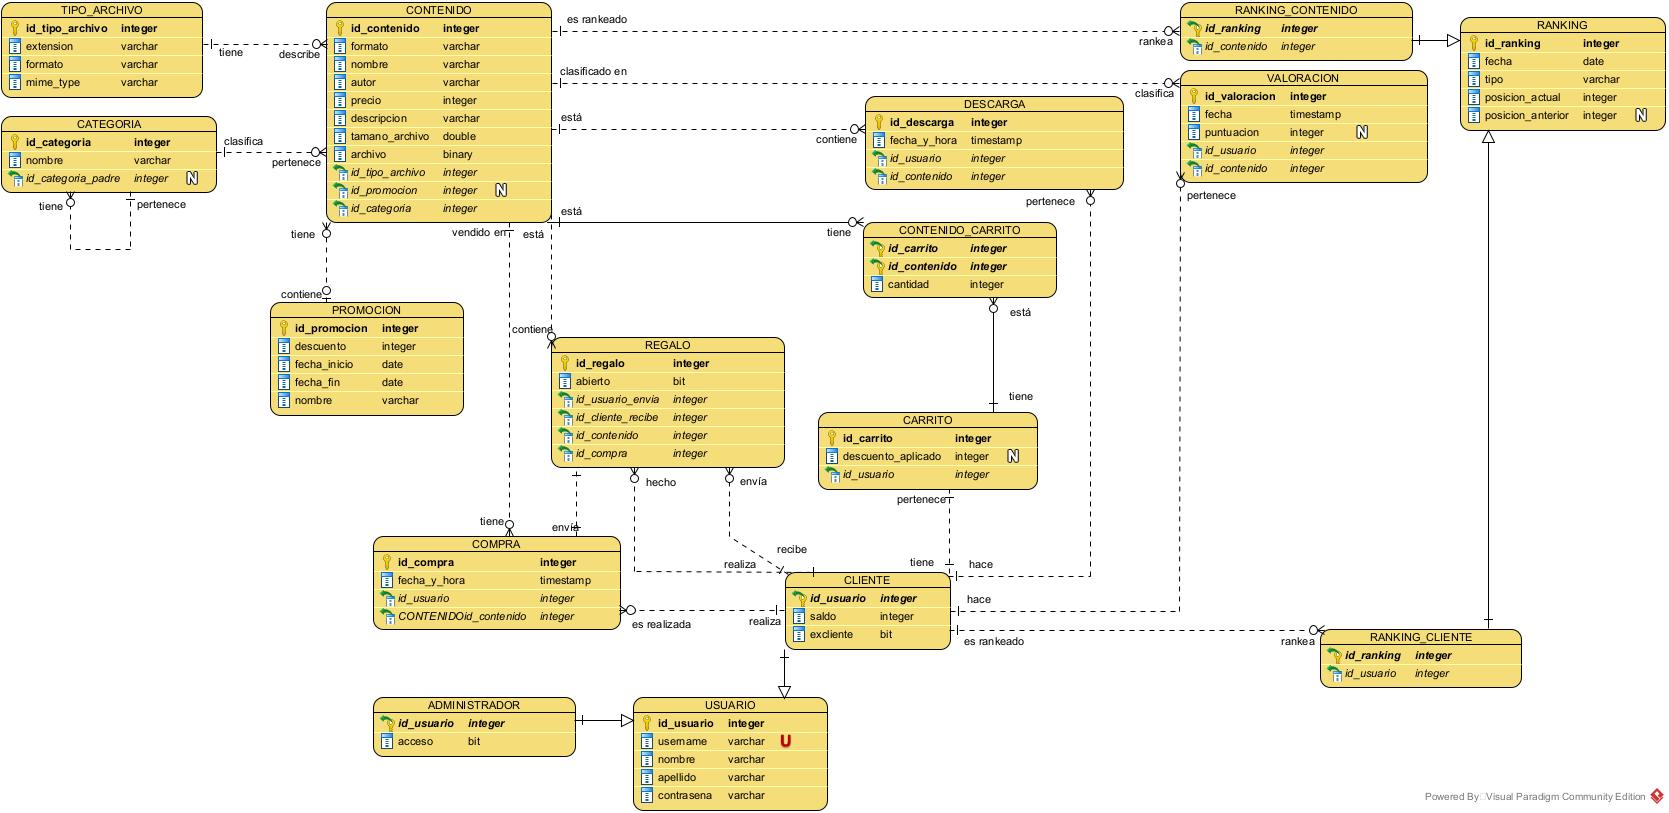
\includegraphics[width=1\textwidth]{Media/4_Disenio/MR.jpg}
    \caption{Modelo Relacional (MR-001) del sistema QuickContentMedia} 
    \label{fig:DiagramaModeloRelacional}
\end{figure}

\textbf{Archivo:} Diagrama del Modelo Relacional (formato Visual Paradigm) \\
\textbf{Link de descarga:} \linkDiagramaModeloRelacional \\

\textbf{Pasos de ejecución:}
\begin{itemize}
    \item Ingresar al repositorio en GitHub usando el link proporcionado y descargar el archivo \texttt{QCM\_MR.vpp}.
    \item En la pestaña Database Modeling/Entity Relationship Model abrir el modelo relacional.
    \item Opcionalmente, descargar el archivo Norm\_pasos.pdf para obtener detalles de la transición del modelo entidad relación (MER-001) al modelo relacional (MR-001).
\end{itemize}

\newpage

\subsection{Diccionario del modelo relacional}

%--------------------------------------------------------------
% DICCIONARIO DE DATOS – MODELO RELACIONAL
% (QuickContentMedia – Versión derivada del MR, sin longitudes VARCHAR)
%--------------------------------------------------------------
\renewcommand{\arraystretch}{1.25}

%--------------------------------------------------------------
\begin{longtable}{|l|l|p{5cm}|p{5cm}|}
\caption{Tabla: \textbf{USUARIO}}\\ \hline
\textbf{Atributo} & \textbf{Tipo de dato} & \textbf{Restricciones} & \textbf{Descripción} \\ \hline
\endfirsthead
\hline \textbf{Atributo} & \textbf{Tipo de dato} & \textbf{Restricciones} & \textbf{Descripción} \\ \hline
\endhead
id\_usuario & integer & PK, NN & Identificador único de cada usuario. \\ \hline
username    & varchar & NN, U  & Nombre de inicio de sesión (único). \\ \hline
nombre      & varchar & NN     & Nombre propio. \\ \hline
apellido    & varchar & NN     & Apellidos. \\ \hline
contrasena  & varchar & NN     & Contraseña cifrada (hash). \\ \hline
\end{longtable}

%--------------------------------------------------------------
\begin{longtable}{|l|l|p{5cm}|p{5cm}|}
\caption{Tabla: \textbf{ADMINISTRADOR}}\\ \hline
\textbf{Atributo} & \textbf{Tipo de dato} & \textbf{Restricciones} & \textbf{Descripción} \\ \hline
\endfirsthead
\hline \textbf{Atributo} & \textbf{Tipo de dato} & \textbf{Restricciones} & \textbf{Descripción} \\ \hline
\endhead
id\_usuario & integer & PK, FK(USUARIO.id\_usuario), NN & Hereda la PK de \textit{USUARIO}. \\ \hline
acceso      & bit     & NN & Indicador de privilegios de gestión. \\ \hline
\end{longtable}

%--------------------------------------------------------------
\begin{longtable}{|l|l|p{5cm}|p{5cm}|}
\caption{Tabla: \textbf{CLIENTE}}\\ \hline
\textbf{Atributo} & \textbf{Tipo de dato} & \textbf{Restricciones} & \textbf{Descripción} \\ \hline
\endfirsthead
\hline \textbf{Atributo} & \textbf{Tipo de dato} & \textbf{Restricciones} & \textbf{Descripción} \\ \hline
\endhead
id\_usuario & integer & PK, FK(USUARIO.id\_usuario), NN & Hereda la PK de \textit{USUARIO}. \\ \hline
saldo       & integer & NN & Saldo vigente para compras (moneda del sistema). \\ \hline
excliente   & bit     & NN & 1 = cuenta cerrada; 0 = activa. \\ \hline
\end{longtable}

%--------------------------------------------------------------
\begin{longtable}{|l|l|p{5cm}|p{5cm}|}
\caption{Tabla: \textbf{TIPO\_ARCHIVO}}\\ \hline
\textbf{Atributo} & \textbf{Tipo de dato} & \textbf{Restricciones} & \textbf{Descripción} \\ \hline
\endfirsthead
\hline \textbf{Atributo} & \textbf{Tipo de dato} & \textbf{Restricciones} & \textbf{Descripción} \\ \hline
\endhead
id\_tipo\_archivo & integer & PK, NN & Identificador único. \\ \hline
extension         & varchar & NN     & Extensión física (ej.\ \texttt{jpg}). \\ \hline
formato           & varchar & NN     & Categoría (\textit{imagen}, \textit{audio}, …). \\ \hline
mime\_type        & varchar & NN     & Tipo MIME oficial. \\ \hline
\end{longtable}

%--------------------------------------------------------------
\begin{longtable}{|l|l|p{5cm}|p{5cm}|}
\caption{Tabla: \textbf{CATEGORIA}}\\ \hline
\textbf{Atributo} & \textbf{Tipo de dato} & \textbf{Restricciones} & \textbf{Descripción} \\ \hline
\endfirsthead
\hline \textbf{Atributo} & \textbf{Tipo de dato} & \textbf{Restricciones} & \textbf{Descripción} \\ \hline
\endhead
id\_categoria       & integer & PK, NN & Identificador de la categoría. \\ \hline
nombre              & varchar & NN     & Nombre de la categoría. \\ \hline
id\_categoria\_padre & integer & FK(CATEGORIA.id\_categoria) & Categoría padre (NULL para nivel raíz). \\ \hline
\end{longtable}

%--------------------------------------------------------------
\begin{longtable}{|l|l|p{5cm}|p{5cm}|}
\caption{Tabla: \textbf{PROMOCION}}\\ \hline
\textbf{Atributo} & \textbf{Tipo de dato} & \textbf{Restricciones} & \textbf{Descripción} \\ \hline
\endfirsthead
\hline \textbf{Atributo} & \textbf{Tipo de dato} & \textbf{Restricciones} & \textbf{Descripción} \\ \hline
\endhead
id\_promocion & integer & PK, NN & Identificador de la promoción. \\ \hline
descuento     & integer & NN & Porcentaje 0–100\,\%. \\ \hline
fecha\_inicio & date    & NN & Inicio de vigencia. \\ \hline
fecha\_fin    & date    & NN & Fin de vigencia. \\ \hline
nombre        & varchar & NN & Nombre de la promoción. \\ \hline
\end{longtable}

%--------------------------------------------------------------
\begin{longtable}{|l|l|p{5cm}|p{5cm}|}
\caption{Tabla: \textbf{CONTENIDO}}\\ \hline
\textbf{Atributo} & \textbf{Tipo de dato} & \textbf{Restricciones} & \textbf{Descripción} \\ \hline
\endfirsthead
\hline \textbf{Atributo} & \textbf{Tipo de dato} & \textbf{Restricciones} & \textbf{Descripción} \\ \hline
\endhead
id\_contenido   & integer & PK, NN & Identificador único del contenido. \\ \hline
formato         & varchar & NN     & Tipo (\textit{video}, \textit{imagen}, …). \\ \hline
nombre          & varchar & NN     & Título o nombre público. \\ \hline
autor           & varchar & NN     & Creador/autores. \\ \hline
precio          & integer & NN     & Precio en la moneda del sistema. \\ \hline
descripcion     & varchar & NN     & Descripción ampliada. \\ \hline
tamano\_archivo & double  & NN     & Tamaño en MB. \\ \hline
archivo         & bytea   & NN     & BLOB o ruta al binario. \\ \hline
id\_tipo\_archivo& integer & FK(TIPO\_ARCHIVO.id\_tipo\_archivo), NN & Tipo físico del archivo. \\ \hline
id\_promocion   & integer & FK(PROMOCION.id\_promocion) & Promoción activa (NULL si no aplica). \\ \hline
id\_categoria   & integer & FK(CATEGORIA.id\_categoria), NN & Categoría asignada. \\ \hline
\end{longtable}

%--------------------------------------------------------------
\begin{longtable}{|l|l|p{5cm}|p{5cm}|}
\caption{Tabla: \textbf{COMPRA}}\\ \hline
\textbf{Atributo} & \textbf{Tipo de dato} & \textbf{Restricciones} & \textbf{Descripción} \\ \hline
\endfirsthead
\hline \textbf{Atributo} & \textbf{Tipo de dato} & \textbf{Restricciones} & \textbf{Descripción} \\ \hline
\endhead
id\_compra     & integer   & PK, NN & Número de transacción. \\ \hline
fecha\_y\_hora & timestamp & NN     & Sello de tiempo de la operación. \\ \hline
id\_usuario    & integer   & FK(USUARIO.id\_usuario), NN & Comprador. \\ \hline
id\_contenido  & integer   & FK(CONTENIDO.id\_contenido) & Contenido adquirido (si sólo se compra de a uno; de lo contrario separar a tabla detalle). \\ \hline
\end{longtable}

%--------------------------------------------------------------
\begin{longtable}{|l|l|p{5cm}|p{5cm}|}
\caption{Tabla: \textbf{REGALO}}\\ \hline
\textbf{Atributo} & \textbf{Tipo de dato} & \textbf{Restricciones} & \textbf{Descripción} \\ \hline
\endfirsthead
\hline \textbf{Atributo} & \textbf{Tipo de dato} & \textbf{Restricciones} & \textbf{Descripción} \\ \hline
\endhead
id\_regalo         & integer & PK, NN & Identificador del regalo. \\ \hline
abierto            & bit     & NN & 1 = abierto por el destinatario. \\ \hline
id\_usuario\_envia & integer & FK(USUARIO.id\_usuario), NN & Remitente. \\ \hline
id\_cliente\_recibe& integer & FK(CLIENTE.id\_usuario), NN & Destinatario. \\ \hline
id\_contenido      & integer & FK(CONTENIDO.id\_contenido), NN & Contenido regalado. \\ \hline
id\_compra         & integer & FK(COMPRA.id\_compra) & Compra asociada (opcional). \\ \hline
\end{longtable}

%--------------------------------------------------------------
\begin{longtable}{|l|l|p{5cm}|p{5cm}|}
\caption{Tabla: \textbf{CARRITO}}\\ \hline
\textbf{Atributo} & \textbf{Tipo de dato} & \textbf{Restricciones} & \textbf{Descripción} \\ \hline
\endfirsthead
\hline \textbf{Atributo} & \textbf{Tipo de dato} & \textbf{Restricciones} & \textbf{Descripción} \\ \hline
\endhead
id\_carrito        & integer & PK, NN & Identificador del carrito. \\ \hline
descuento\_aplicado& integer &        & Porcentaje total de descuento aplicado. \\ \hline
id\_usuario        & integer & FK(USUARIO.id\_usuario), NN & Propietario del carrito. \\ \hline
\end{longtable}

%-------------------------------------------------------------
\newpage
\begin{longtable}{|l|l|p{5cm}|p{5cm}|}
\caption{Tabla puente: \textbf{CONTENIDO\_CARRITO}}\\ \hline
\textbf{Atributo} & \textbf{Tipo de dato} & \textbf{Restricciones} & \textbf{Descripción} \\ \hline
\endfirsthead
\hline \textbf{Atributo} & \textbf{Tipo de dato} & \textbf{Restricciones} & \textbf{Descripción} \\ \hline
\endhead
id\_carrito   & integer & PK\textsuperscript{*}, FK(CARRITO.id\_carrito), NN & Carrito asociado. \\ \hline
id\_contenido & integer & PK\textsuperscript{*}, FK(CONTENIDO.id\_contenido), NN & Contenido incluido. \\ \hline
cantidad      & integer & NN & Cantidad de unidades. \\ \hline
\multicolumn{4}{l}{\footnotesize * Clave primaria compuesta (id\_carrito, id\_contenido).} \\
\end{longtable}

%--------------------------------------------------------------
\begin{longtable}{|l|l|p{5cm}|p{5cm}|}
\caption{Tabla: \textbf{DESCARGA}}\\ \hline
\textbf{Atributo} & \textbf{Tipo de dato} & \textbf{Restricciones} & \textbf{Descripción} \\ \hline
\endfirsthead
\hline \textbf{Atributo} & \textbf{Tipo de dato} & \textbf{Restricciones} & \textbf{Descripción} \\ \hline
\endhead
id\_descarga  & integer   & PK, NN & Identificador de la descarga. \\ \hline
fecha\_y\_hora& timestamp & NN & Momento exacto de la acción. \\ \hline
id\_usuario   & integer   & FK(USUARIO.id\_usuario), NN & Usuario que descarga. \\ \hline
id\_contenido & integer   & FK(CONTENIDO.id\_contenido), NN & Contenido descargado. \\ \hline
\end{longtable}

%--------------------------------------------------------------
\begin{longtable}{|l|l|p{5cm}|p{5cm}|}
\caption{Tabla: \textbf{VALORACION}}\\ \hline
\textbf{Atributo} & \textbf{Tipo de dato} & \textbf{Restricciones} & \textbf{Descripción} \\ \hline
\endfirsthead
\hline \textbf{Atributo} & \textbf{Tipo de dato} & \textbf{Restricciones} & \textbf{Descripción} \\ \hline
\endhead
id\_valoracion & integer   & PK, NN & Identificador de la valoración. \\ \hline
fecha          & timestamp & NN & Fecha/hora de emisión. \\ \hline
puntuacion     & integer   & NN & Nota 1–10 otorgada. \\ \hline
id\_usuario    & integer   & FK(USUARIO.id\_usuario), NN & Autor de la valoración. \\ \hline
id\_contenido  & integer   & FK(CONTENIDO.id\_contenido), NN & Contenido valorado. \\ \hline
\end{longtable}

%-------------------------------------------------------------
\newpage
\begin{longtable}{|l|l|p{5cm}|p{5cm}|}
\caption{Tabla: \textbf{RANKING}}\\ \hline
\textbf{Atributo} & \textbf{Tipo de dato} & \textbf{Restricciones} & \textbf{Descripción} \\ \hline
\endfirsthead
\hline \textbf{Atributo} & \textbf{Tipo de dato} & \textbf{Restricciones} & \textbf{Descripción} \\ \hline
\endhead
id\_ranking        & integer & PK, NN & Identificador del ranking. \\ \hline
fecha              & date    & NN & Fecha de generación. \\ \hline
tipo               & varchar & NN & Criterio (\textit{descargas}, \textit{puntuación}). \\ \hline
posicion\_actual   & integer & NN & Posición evaluada actualmente. \\ \hline
posicion\_anterior & integer &     & Posición en periodo previo (NULL si no aplica). \\ \hline
\end{longtable}

%--------------------------------------------------------------
\begin{longtable}{|l|l|p{5cm}|p{5cm}|}
\caption{Tabla puente: \textbf{RANKING\_CONTENIDO}}\\ \hline
\textbf{Atributo} & \textbf{Tipo de dato} & \textbf{Restricciones} & \textbf{Descripción} \\ \hline
\endfirsthead
\hline \textbf{Atributo} & \textbf{Tipo de dato} & \textbf{Restricciones} & \textbf{Descripción} \\ \hline
\endhead
id\_ranking   & integer & PK\textsuperscript{*}, FK(RANKING.id\_ranking), NN & Ranking al que pertenece. \\ \hline
id\_contenido & integer & PK\textsuperscript{*}, FK(CONTENIDO.id\_contenido), NN & Contenido posicionado. \\ \hline
\multicolumn{4}{l}{\footnotesize * Clave primaria compuesta (id\_ranking, id\_contenido).} \\
\end{longtable}

%--------------------------------------------------------------
\begin{longtable}{|l|l|p{5cm}|p{5cm}|}
\caption{Tabla puente: \textbf{RANKING\_CLIENTE}}\\ \hline
\textbf{Atributo} & \textbf{Tipo de dato} & \textbf{Restricciones} & \textbf{Descripción} \\ \hline
\endfirsthead
\hline \textbf{Atributo} & \textbf{Tipo de dato} & \textbf{Restricciones} & \textbf{Descripción} \\ \hline
\endhead
id\_ranking & integer & PK\textsuperscript{*}, FK(RANKING.id\_ranking), NN & Ranking al que pertenece. \\ \hline
id\_usuario & integer & PK\textsuperscript{*}, FK(USUARIO.id\_usuario), NN & Cliente posicionado. \\ \hline
\multicolumn{4}{l}{\footnotesize * Clave primaria compuesta (id\_ranking, id\_usuario).} \\
\end{longtable}